\documentclass[a4paper]{article}
\usepackage[utf8]{inputenc}
\usepackage[symbol]{footmisc}
\usepackage{geometry}
\geometry{left=1.2in, right=1.2in, bottom=1.5in}
\setlength{\parindent}{0pt}
\setlength{\parskip}{0.5em}
\usepackage{enumitem}
\setlist{topsep=-0.25mm, itemsep=-0.25mm}
\usepackage{ragged2e}
\usepackage{xspace}
\usepackage[dvipsnames]{xcolor}
\usepackage{fancyhdr}
\usepackage{hyperref}
\usepackage{graphicx}
\usepackage{float}
\graphicspath{ {./} }
\newcommand{\latex}{\LaTeX\xspace}
\newcommand{\tex}{\TeX\xspace}
\title{\latex Starter Pack}
\author{190050062-190050116}
\date{August 24 2020}

\pagestyle{fancy}
\fancyhf{}
\rhead{Software Systems Laboratory}
\lhead{190050062-190050116}
\cfoot{Page \thepage}
\renewcommand{\footrulewidth}{1pt}

\begin{document}

\maketitle
\tableofcontents
\thispagestyle{empty}
\setcounter{page}{0}
\newpage

\section{Introduction}
\latex (most popularly pronounced lay-tech; sometimes laa-tech) is an incredibly efficient office tool to typeset professional looking technical documents and reports. You will certainly find it useful to write assignments, format your resume, and more generally, to make everything you do look cooler.\par
\latex, like HTML, is a \textbf{markup language}. It's part of the \tex typesetting system created by the immortal Donald Knuth. The presentation of the content depends on the properties of the tags it is wrapped in. For more involved typesetting purposes, this gives it a clear edge over mainstream word processors like MS-Word: in Word, \textit{what you see is what you get}, and getting what you want can be insanely tough.\par
Here's how it works: you write your markup commands in the source file, which has a \texttt{.tex} extension. You need ``software", or formally, a \tex distribution, to actually typeset them into a format suitable for distribution, which is generally a pdf. The most popular distribution to install on your machine is TeX Live; MikTeX is an alternative. You could also work online with Overleaf - no installations, and a ridiculously straightforward workflow. This is ideal for smaller projects. Weigh your options \href{https://www.latex-project.org/get/}{here}. Yes, a hyperlink!\par
\latex allows us to write complex mathematical equations without much fuss; its environments save us the hassle of organising large documents manually; with \latex we can showcase code and render almost any scientific illustration. \latex is paradise for anyone who works in STEM. Once you have experience, you can typeset assignments, papers, articles and theses with unprecedented ease.\par
In this assignment, we will explore and demonstrate some features that often prove themselves useful for several purposes.\par
\begin{large}
In this introductory section, we have also seen how we can format text. For instance, we can make text bold, italicized, colour it, or manipulate its size, and even toggle between alignments!\par
\end{large}
\begin{flushright}
\textcolor{Sepia}{{\LARGE C}{\large ARPE} {\LARGE D}{\large IEM!}}
\end{flushright}
\begin{figure}[H]
\centering
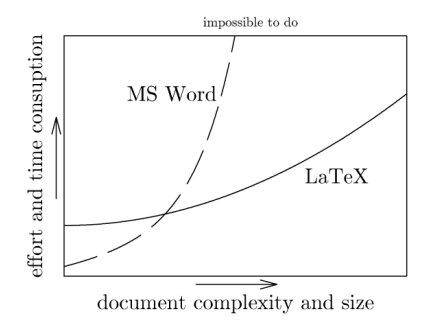
\includegraphics[scale=0.5]{ease-graph.png}
\caption{The graph of Marko Pinteric is spot on}
\end{figure}
\section{Basic Document Formatting}
In STEM, brevity is highly valued. You want to put forth your arguments as crisply as possible. Of course, sometimes a rather long clarification may be in order\renewcommand*{\thefootnote}{\arabic{footnote}}\footnote{Footnotes are a classy way to do that. Making footnotes is fairly simple in \latex.}, however, it is better to stick to the central theme and not disrupt the flow. In order to make your point, lists are often the cleanest option.\par
\paragraph{Features we demonstrate}
\begin{itemize}
\item Making a title and table of contents
\item Organising the document into sections
\item Setting up the page layout
\item Designing our custom header and footer
\item Formatting text
\item Making (nested) lists
\begin{enumerate}
    \item itemize
    \item enumerate
    \item description
\end{enumerate}
\item Footnotes
\item Typesetting mathematics
\item Theorem and Proof environments
\item Hyperlinks and cross reference within the document
\item Custom environments
\item Algorithms and code
\item Inserting images
\item Drawing tables
\renewcommand*{\thefootnote}{\fnsymbol{footnote}}
\item Citations\footnote[2]{using BibTeX, which automatically takes care of the bibliography formatting}
\renewcommand*{\thefootnote}{\arabic{footnote}}
\end{itemize}
In order to make your list appear more concise, you can specify the \texttt{itemsep} parameter as an optional argument to the environment. You will need \texttt{enumitem} package for that.\par
Descriptive lists are sometimes handy:\par
\begin{description}
\item[CS207] Discrete Structures
\item[CS213] Data Structures and Algorithms
\item[CS215] Data Analysis and Interpretation
\item[CS251] Software Systems Lab
\item[CS293] Data Structures and Algorithms Lab
\end{description}
\paragraph{The Page Layout}\mbox{}\\\mbox{}\\
The paper size for this document is A4. The left and right margins are 1.2 inches each; the lower margin is 1.5 inches. The \texttt{geometry} package is very convenient to set up and manipulate these dimensions.\mbox{}\\\mbox{}\\\mbox{}\\
\section{Mathematics}
\section{Computer Science}
\section{Utilities}
\end{document}
